\section{Convolutional Neural Network}
\label{sec:03_Convolutional_Neural_Network}

Building upon the dataset established in the preceding Section \ref{sec:02_Navier-Stokes_Simulation}, this Section introduces a surrogate model designed to approximate the results of CFD simulations with a significant reduction in computational time.\\

Our approach is centered on a \textbf{Convolutional Neural Network (CNN)}, a deep learning architecture adept at learning the complex physical relationships that govern aerodynamic performance directly from simulation data. \\

Specifically, the network is designed to predict the lift coefficient ($C_L$) as a function of three key inputs: 
\begin{enumerate}
    \item the airfoil shape, represented as a \textbf{Signed Distance Function};
    \item the angle of attack ($\alpha$);
    \item the Reynolds number ($\mathrm{Re}$).
\end{enumerate}
By training on the generated simulation results, the CNN effectively learns to emulate the fluid dynamics solver, enabling near-instantaneous predictions.\\

The following sections will provide a comprehensive overview of this CNN model, from its underlying mathematical principles to its custom implementation designed for high-performance computing.

% ===================================================================
% MATHEMATICAL BACKGROUND
% ===================================================================

\subsection{Mathematical Background}

This section details the mathematical foundations of our surrogate modeling approach.\\
We first introduce the \textbf{Signed Distance Function (SDF)}, which transforms the airfoil's complex geometry into a structured grid suitable for a neural network. We then provide a comprehensive breakdown of the \textbf{Convolutional Neural Network architecture}, explaining the mathematical operations within each layer and the physics-informed training algorithm used to learn the mapping from geometry and flow conditions to the aerodynamic lift coefficient.

\subsubsection{Geometric Representation with Signed Distance Function}
\label{sec:03_SDF}

To construct a deep learning model capable of predicting aerodynamic coefficients, we need a robust method for representing the geometry of the airfoil $\Omega \subset \mathbb{R}^2$ and its boundary $\partial\Omega$ in a format suitable for Convolutional Neural Networks. Traditional boundary representations, such as coordinates of boundary points, are challenging to process with standard convolutional operators because they lack fixed spatial grids. To address this limitation, we represent the airfoil geometry using a \textbf{Signed Distance Function}, obtaining for each airfoil the result shown in Figure \ref{fig:SDF}.\\

\begin{figure}[h]
    \centering
    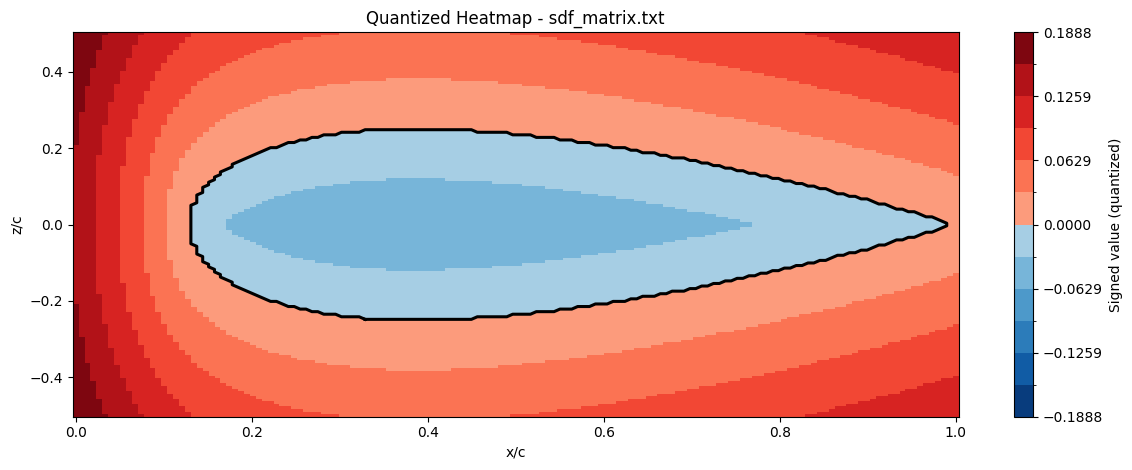
\includegraphics[width=0.65\linewidth]{Images//Chapter03/SDF.png}
    \caption{The Signed Distance Field representation of a NACA 0012 airfoil, discretized on a uniform grid. Negative values (blue) correspond to the airfoil interior, positive values (red) to the exterior while the boundary is represented by the zero-level contour (black line).}
    \label{fig:SDF}
\end{figure}

The SDF $\Phi: \mathbb{R}^2 \to \mathbb{R}$ maps any point $P = (x, z)$ in the spatial domain to its signed distance from the boundary $\partial\Omega$:
\begin{equation}
    \Phi(P) = \begin{cases}
        -d(P, \partial\Omega) & \text{if } P \in \Omega \\
        \phantom{-} d(P, \partial\Omega) & \text{if } P \notin \Omega
    \end{cases}
    \label{eq:sdf_definition}
\end{equation}
where $d(P, \partial\Omega)$ represents the Euclidean distance from the point $P$ to the boundary $\partial\Omega$:
\begin{equation}
    d(P, \partial\Omega) = \inf_{Q \in \partial\Omega} \|P - Q\|_2
    \label{eq:distance_to_boundary}
\end{equation}
Using this definition, the boundary of the airfoil is implicitly defined as the zero-level set of the function:
\begin{equation}
    \partial\Omega = \{P \in \mathbb{R}^2 \mid \Phi(P) = 0\}
\end{equation}
while the interior corresponds to negative values ($\Phi(P) < 0$) and the exterior to positive values ($\Phi(P) > 0$).\\

In our numerical implementation, the boundary $\partial\Omega$ is defined as a closed polygon composed of an ordered set of $n$ vertices $\{V_0, V_1, \dots, V_{n-1}\}$.\\
To guarantee scale invariance, the coordinates of the airfoil profile are first normalized by the chord length $c$, defined as the Euclidean distance between the leading edge point $(x_{\min}, z|_{x_{\min}})$ and the trailing edge point $(x_{\max}, z|_{x_{\max}})$:
\begin{equation}
 c = \sqrt{(x_{\max} - x_{\min})^2 + (z_{\text{at } x_{\max}} - z_{\text{at } x_{\min}})^2}
\end{equation}
where $x_{\max}$, $x_{\min}$, $z_{\max}$, and $z_{\min}$ are the extreme coordinates computed over the boundary vertices. Each vertex is then scaled by dividing its coordinates by $c$:
\begin{equation}
    V_i = \left(\frac{x_{V_i}}{c}, \frac{z_{V_i}}{c}\right)
\end{equation}
The boundary $\partial\Omega$ is then represented as the union of $n$ linear segments $S_i = [V_i, V_{i+1}]$ (with $V_n = V_0$). The minimum distance from a grid point $P$ to the boundary $\partial\Omega$ is computed by finding the minimum distance to each individual segment $S_i$:
\begin{equation}
    d(P, \partial\Omega) = \min_{i=0, \dots, n-1} d(P, S_i)
\end{equation}
For a given segment $S_i$ defined by the endpoints $A = V_i$ and $B = V_{i+1}$, any point on the infinite line passing through $A$ and $B$ can be parameterized as $P(t) = A + t(B-A)$ for $t \in \mathbb{R}$. The orthogonal projection of the point $P$ onto this line is obtained by minimizing the distance $\|P - P(t)\|^2$, which yields the projection parameter:
\begin{equation}
    t^* = \frac{(P - A) \cdot (B - A)}{\|B - A\|_2^2}
    \label{eq:03_orthogonal_projection}
\end{equation}
To restrict the projection to the finite line segment $S_i$, $t^*$ is clamped to the interval $[0, 1]$:
\begin{equation}
    t = \max\left(0, \min\left(1, t^*\right)\right)
    \label{eq:03_clamping}
\end{equation}
The projection point on the segment is then $P_{\text{proj}} = A + t(B-A)$, and the distance to the segment is:
\begin{equation}
    d(P, S_i) = \|P - P_{\text{proj}}\|_2
\end{equation}

To determine the sign of the distance field, we implement the \textbf{Winding Number Algorithm} to check whether a grid point $P$ lies inside or outside the closed boundary. The winding number $wn(P)$ computes the number of times the boundary curve wraps around the point $P$. For a closed polygon, it is computed by casting a horizontal ray starting from $P$ and pointing in the positive $x$-direction, and counting the signed crossings of this ray with the polygon edges:
\begin{itemize}
    \item[-] an \textbf{upward crossing} occurs if an edge $S_i = [V_i, V_{i+1}]$ crosses the horizontal ray from below, i.e., $V_{i, z} \le z_P < V_{i+1, z}$ and $P$ lies to the left of the directed line segment;
    \item[-] a \textbf{downward crossing} occurs if an edge $S_i$ crosses the horizontal ray from above, i.e., $V_{i+1, z} \le z_P < V_{i, z}$ and $P$ lies to the right of the directed line segment.
\end{itemize}
The relative position of the point $P$ with respect to the directed segment $[A, B]$ is determined mathematically using the 2D cross product:
\begin{equation}
    \text{cross}(P, A, B) = (A_x - x_P)(B_z - z_P) - (B_x - x_P)(A_z - z_P)
    \label{eq:cross_product}
\end{equation}
If $\text{cross}(P, A, B) > 0$, the point $P$ lies to the left of the directed segment, whereas if $\text{cross}(P, A, B) < 0$, it lies to the right. The winding number is incremented by 1 for every upward crossing and decremented by 1 for every downward crossing. A point $P$ is strictly inside the domain $\Omega$ if and only if the total winding number is non-zero:
\begin{equation}
    P \in \Omega \iff wn(P) \ne 0
\end{equation}
Once the signed distance is computed for any point, we project it onto a discrete uniform grid. The spatial domain is discretized into a Cartesian grid of size $N \times N = 150 \times 150$ over the bounding box $[X_{\min}, X_{\max}] \times [Z_{\min}, Z_{\max}]$, with:
\begin{equation}
    X_{\min} = -0.15, \quad X_{\max} = 1.01, \quad Z_{\min} = -0.12, \quad Z_{\max} = 0.12
\end{equation}
The grid spacing is defined by:
\begin{equation}
    \Delta x = \frac{X_{\max} - X_{\min}}{N-1}, \quad \Delta z = \frac{Z_{\max} - Z_{\min}}{N-1}
\end{equation}
For each grid node indexed by $(row, col)$ for $row, col = 0, \dots, N-1$, the corresponding spatial coordinates are given by:
\begin{equation}
    x_{col} = X_{\min} + col \cdot \Delta x, \quad z_{row} = Z_{\max} - row \cdot \Delta z
\end{equation}
This discretized representation yields a 2D matrix of shape $150 \times 150$, where each entry contains the signed distance value. This matrix provides a spatially structured representation of the geometry that preserves boundary details, making it perfectly suited as an input to the convolutional branch of the neural network.\\

\subsubsection{Convolutional Neural Networks for Aerodynamic Prediction}

The architecture of our \textbf{Convolutional Neural Network} is designed as a multi-input model to effectively process both the spatial geometric data and the scalar physical parameters. A high-level schematic of this design, inspired by the model presented by \cite{Cuozzo2026AIDriven}, is depicted in Figure \ref{fig:cnn_architecture}.\\

\begin{figure}[H]
    \centering
    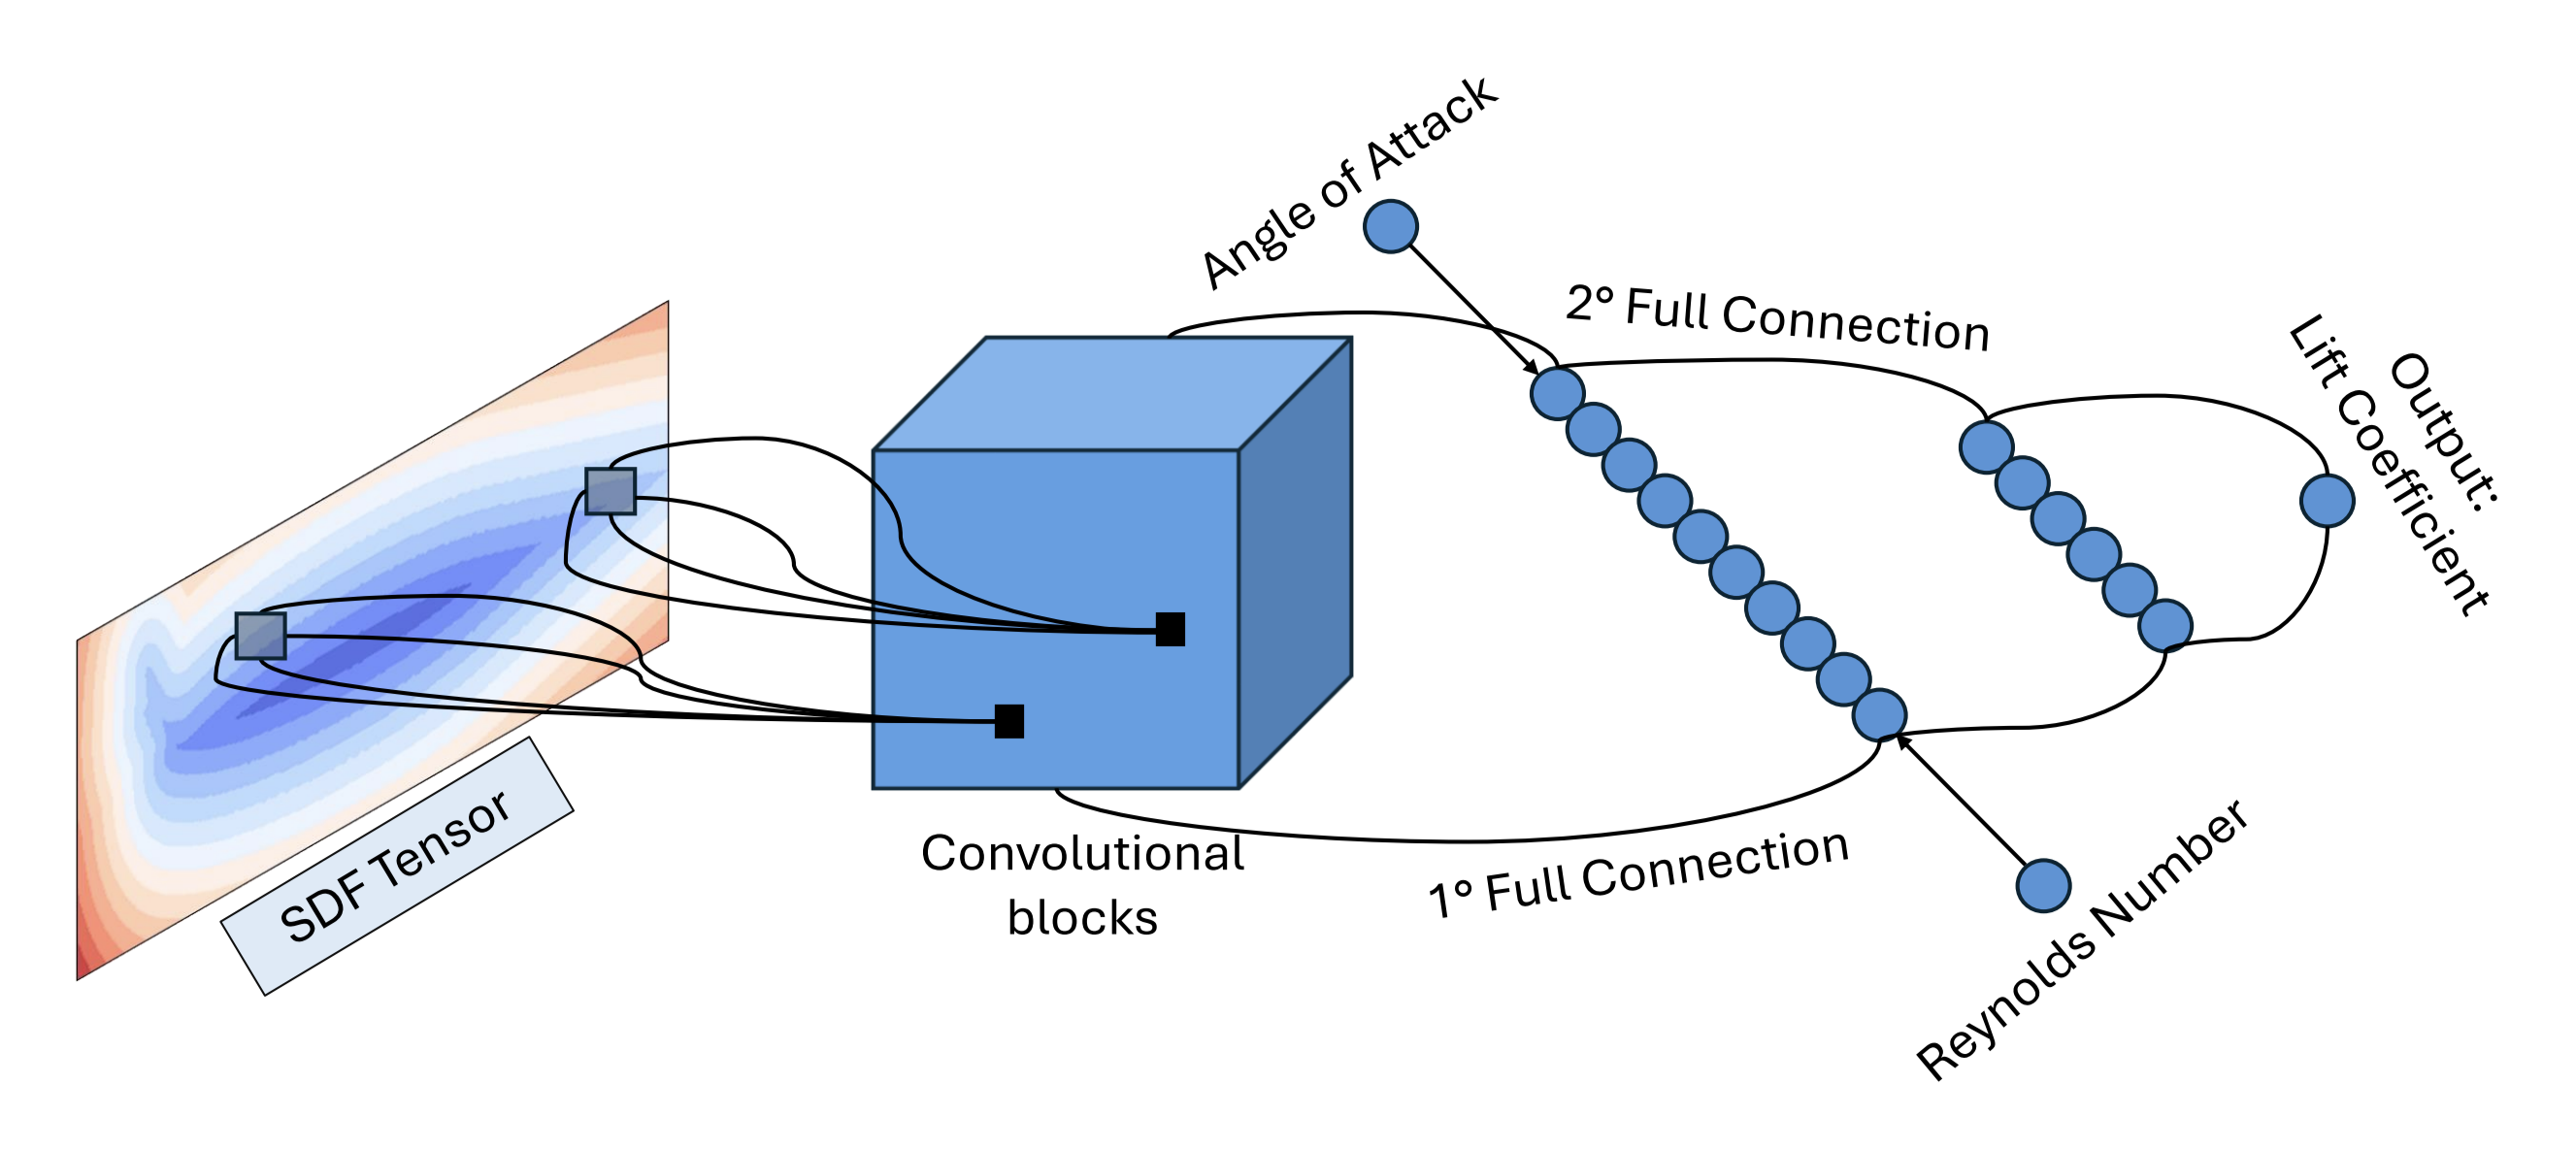
\includegraphics[width=0.8\linewidth]{Images/Chapter03/cnn_architecture.png}
    \caption{Architecture of the Convolutional Neural Network used for aerodynamic prediction.}
    \label{fig:cnn_architecture}
\end{figure}

The network is logically divided into three main components:\\ 
\begin{enumerate}[itemsep=2ex]
    \item a convolutional feature extractor, responsible for interpreting the airfoil geometry. It accepts the 2D SDF matrix as input and processes it through a series of \texttt{Conv2DLayer}s, each followed by a \texttt{LeakyReLULayer} activation. This stack of layers hierarchically extracts relevant spatial features, such as leading-edge curvature and surface details. The resulting multi-channel feature maps are then transformed into a one-dimensional vector by a \texttt{FlattenLayer}, producing a learned representation of the airfoil's shape;
    \item a feature fusion stage, in which, the flattened geometric feature vector from the convolutional branch is concatenated with the scalar physical parameters (the angle of attack and the Reynolds number) tensor using a \texttt{ConcatenateLayer}. This creates a single feature vector that contains comprehensive information about both the airfoil's shape and the current flow conditions;
    \item finally the unified vector is passed to the regression head, which consists of a sequence of \texttt{DenseLayer}s. This fully-connected network maps the combined high-level features to a single scalar output, which represents the predicted lift coefficient, $C_L$.
\end{enumerate}

\paragraph{Convolutional Layer}

The \textbf{Convolutional Layer} (\texttt{Conv2DLayer}) is an operator specifically designed to process grid-like data such as the 2D SDF. Its primary function is to detect local spatial patterns within the input by applying a set of learnable filters. The difference with the dense layer, which treats all input pixels independently, is that a convolutional layer preserves the spatial relationship between pixels by operating on localized neighborhoods.\\

At its core, the operation is a discrete 2D convolution, which can be understood as a \textit{sliding window dot product}. A small matrix of learnable weights, known as the kernel ($K$), slides over the input feature map ($I$). At each position, an element-wise multiplication between the kernel and the overlapping region of the input is performed, and the results are summed up to produce a single pixel in the output feature map ($O$).\\

For a single-channel input $I$ of size $H\times W$ and a kernel of size $F\times F$, the value of the output $O$ at position $(i,j)$ is given by:
\begin{equation}
    O(i,j)=\sum_{m=0}^{F-1}\sum_{n=0}^{F-1}I(i-m,j-n)\cdot K(m,n)+b
    \label{eq:convolutional_sum}
\end{equation}
where $b$ is a learnable scalar bias term applied to the entire output feature map.\\

The key principle here is parameter sharing: the \textit{same} kernel $K$ and bias $b$ are used across all positions of the input, allowing the network to detect the same feature regardless of where it appears in the SDF\footnote{In more details, if the kernel learns to recognize a leading edge curve of a profile, it will successfully detect the curve whether it appears at the top of the grid or in a bottom corner.}.\\

In deep networks, layers typically process multi-channel inputs. If the input feature map has $C_{in}$ channels\footnote{This is not our case, since in the SDF we have only one input channel ($C_{in}=1$).}, the kernel must be three-dimensional, with a size of $F\times F\times C_{in}$. The convolution is then performed across all channels simultaneously. The results from each channel are then summed together to produce a single value for the 2D output map.\\

To generate an output with $C_{out}$ feature maps, we simply apply $C_{out}$ independent kernels. Each kernel is responsible for learning a different spatial feature, allowing the layer to build a complete representation of the input geometry.\\

The behavior of the convolution is controlled by two hyperparameters:\\
\begin{itemize}[itemsep=2ex]
    \item[-] the stride ($S$) defines the step size the kernel matrix as it traverses the input grid. While a unit stride ($S=1$) evaluates adjacent localized neighborhoods sequentially, a stride of $S > 1$ skips spatial coordinates, downsampling the spatial resolution of the resulting feature map;
    \item[-] padding ($P$)\footnote{In our implementation, padding is set to $0$.} consists in appending a perimeter of zero-valued elements around the input grid boundaries. This can be used to control the output dimensions and mitigate the loss of information at the edges.
\end{itemize}
\vspace{2ex}
The dimensions of the output feature map ($H_{out}\times W_{out}$) are determined by the input dimensions ($H_{in}\times W_{in}$), the kernel size ($F$), the stride ($S$) and the padding ($P$) using the following formula:
\begin{equation}
    W_{out}=\frac{W_{in}-F+2P}{S}+1\quad\text{and}\quad H_{out}=\frac{H_{in}-F+2P}{S}+1
    \label{eq:03_convol}
\end{equation}
From an implementation perspective, this operation is typically realized as a set of nested loops that iterate over each position in the output map, each element of the kernel, and each input channel, performing the required multiply-accumulate operations\footnote{We will explain in a better way highlighting our \cpp implementation in Section \ref{sec:03_conv} regarding our implementation in \cpp}.

\paragraph{Non-Linear Activation (Leaky ReLU)}

After each \texttt{Conv2DLayer} or \texttt{DenseLayer} performs its linear operation, an activation function applies a non-linear transformation element-wise to its output. Without this, a deep neural network, regardless of its number of layers, would behave as a single, large linear model. The introduction of non-linearity is what gives the network its power to approximate arbitrarily complex, non-linear relationships, such as the one between airfoil geometry and lift coefficient.\\

In this project, a \textbf{Leaky Rectified Linear Unit} (Leaky ReLU) is implemented as the \texttt{LeakyReLULayer}. This function, shown in Figure \ref{fig:03_relu}, is a popular and effective choice in modern deep learning due to its computational efficiency and its ability to mitigate some of the common problems encountered during training.\\

\begin{figure}[h!]
    \centering
    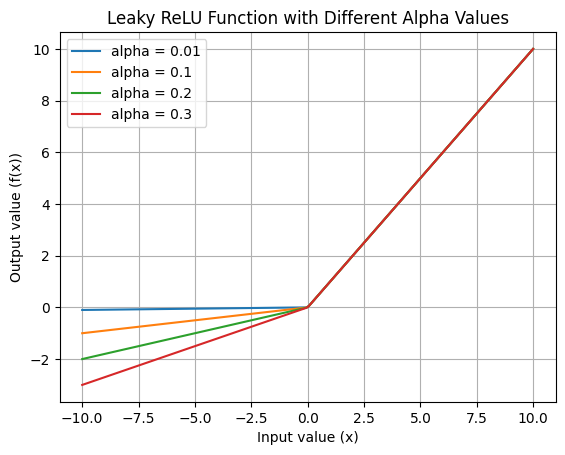
\includegraphics[width=0.4\linewidth]{Images/Chapter03/relu.png}
    \caption{Example of Leaky ReLU function with different $\alpha$.}
    \label{fig:03_relu}
\end{figure}

The Leaky ReLU function is defined mathematically as:
\begin{equation}
    \text{LeakyReLU(x)}=\begin{cases}
        x & \text{ if } x>0\\
        \alpha x&\text{ if } x\le 0
    \end{cases}
    \label{eq:03_leaky_relu}
\end{equation}
where $\alpha$ is a small, positive constant (a hyperparameter, typically set to a value like $0.01$).\\

The function behaves as a simple identity for all positive input values. For negative input values, instead of mapping them to zero like the standard ReLU function, it allows a small, non-zero gradient to pass through.\\

The primary advantage of the Leaky ReLU over the standard ReLU is its handling of negative inputs. In a standard ReLU, if a neuron's input is consistently negative, its gradient will always be zero. This means the neuron's weights will never be updated, and it can effectively "die", ceasing to contribute to the network's learning process. The Leaky ReLU prevents this "dying ReLU" problem by ensuring that a small gradient always exists, even for negative inputs.\\

From the backpropagation algorithm, the gradient of the Leaky ReLU is simple and computationally inexpensive to calculate:
\begin{equation}
    \frac{d}{dx}\text{LeakyReLU(x)}=\begin{cases}
        1 & \text{ if } x>0\\
        \alpha &\text{ if } x\le 0
    \end{cases}
    \label{eq:03_derivative_leaky_relu}
\end{equation}

During the backward pass of training, this straightforward derivative is used to scale the incoming gradient from the subsequent layer:
\begin{itemize}
    \item[-] if the input to the activation function was positive during the forward pass, the gradient passes through unchanged;
    \item[-] if it was negative, the gradient is scaled down by the factor $\alpha$.
\end{itemize}
This simple conditional check makes the backward pass for the \texttt{LeakyReLULayer} extremely fast, contributing to the overall efficiency of the training process.

\paragraph{Structural Layers}
\label{sec:03_struct_layer}

After the convolutional network has extracted a hierarchy of spatial features, the resulting multi-channel feature maps must be prepared for integration with the scalar parameters and for final processing by the regression head. This preparation is handled by two complementary \textbf{structural layers}, the \texttt{FlattenLayer} and the \texttt{ConcatenateLayer}, that are parameter-free: they do not contain any learnable weights or biases since their sole purpose is to rearrange data tensors.\\

\textbf{Flatten Layer}\\

The \texttt{FlattenLayer} links the convolutional layers and the fully-connected layers. Convolutional layers output a 4D tensor with a shape of \texttt{[Batch Size, Channels, Height, Width]}, preserving spatial information. However, dense layers require their input to be a 2D tensor of shape \texttt{[Batch Size, Features]}, where each row is a one-dimensional vector representing a single sample.\\

The flatten operation reshapes an input tensor $T_{in}$ with dimensions $[B\times C_{out}\times H_{out}\times W_{out}]$ into an output tensor $T_{out}$ with dimensions $[B\times D]$, where the new feature dimension $D$ is the product of the input's channel, height and width dimensions:
\begin{equation}
    D=C_{out}\times H_{out}\times W_{out}
\end{equation}
During the forward pass, this is a straightforward memory rearrangement.\\
During  the backward pass for backpropagation, the \texttt{FlattenLayer} performs the inverse operation: it receives an incoming gradient tensor of shape $[B\times D]$ and reshapes it back to the original 4D shape $[B\times C_{out}\times H_{out}\times W_{out}]$. This ensures that the gradients are correctly propagated back to the preceding convolutional layer in the required spatial format.\\

\textbf{Concatenate Layer}\\

Once the geometric features have been flattened into a vector, they must be combined with the scalar physical parameters by the \texttt{ConcatenateLayer}, that takes multiple input tensors and joins them together along a specified axis\footnote{In our case, this is the feature axis (axis 1)}.\\

Mathematically, given the flattened geometric feature tensor $T_{flat}$ of shape $[B\times D_1]$ and the scalar input tensor $T_{scalar}$ (containing angle of attack and Reynolds number) of shape $[B\times D_2]$, the Concatenate Layer produces an output tensor $T_{concat}$ of shape $[B\times (D_1+D_2)]$. This operation creates a unified feature vector that encodes both geometric and physical information for the network to make a prediction.\\

During backpropagation, the process is reversed. The incoming gradient tensor is split according to the original input sizes:
\begin{itemize}
    \item[-] the first $D_1$ elements of the gradient vector are passed back to the \texttt{FlattenLayer}'s branch;
    \item[-] the $D_2$ elements corresponding to the scalar inputs are also computed, although they terminate at the input layer.
\end{itemize}
\vspace{2ex}
After this fusion step, the resulting unified tensor is ready to be processed by the final regression head of the network.

\paragraph{Dense Layer and final regression}
\label{sec:03_dense_layer}

The final computational stage of the network is handled by the\textbf{ Dense Layer} (\texttt{DenseLayer}), known as a fully-connected layer. Its role is to learn the final mapping from the feature space to the target scalar value (the lift coefficient $C_L$).\\

A dense layer applies a linear transformation to its input vector. For an input vector $\mathbf x\in \mathbb R^{D_{in}}$, the layer computes an output vector $\mathbf y\in \mathbb R^{D_{out}}$ using a learnable weight matrix $W\in \mathbb R^{D_{out}\times D_{in}}$ and a learnable bias vector $\mathbf b\in\mathbb R^{D_{out}}$. The operation is defined as:
\begin{equation}
    \mathbf y=W\mathbf x+\mathbf b
\end{equation}
This operation performs a weighted sum of all input features to compute each output feature. Every neuron in the input layer is connected to every neuron in the output layer, allowing the network to model complex interactions between all elements of the input feature vector.\\

This layer is used in the regression head, which consists of a sequence of \texttt{DenseLayer}s, each followed by a \texttt{LeakyReLULayer} activation:
\begin{itemize}
    \item[-] the initial dense layers take concatenated feature vector as input. Their purpose is to find and amplify the non-linear correlations between the learned geometric features from the SDF and the raw physical parameters ($\alpha$ and $\mathrm{Re}$);
    \item[-] the last layer is configured to have a single output neuron ($D_{out}=1$) and does not have a subsequent activation function. This single neuron's output directly corresponds to the network's prediction for the lift coefficient ($C_L$).
\end{itemize}
\vspace{2ex}
During the backward pass, the dense layer must compute three distinct gradients based on the incoming gradient from the subsequent layer $\frac{\partial L}{\partial \mathbf y}$, where $L$ is the loss:
\begin{itemize}
    \item[-] the gradient with respect to the weights ($W$) is calculated as the outer product of the incoming gradient and the layer's input vector from the forward pass:
    \begin{equation}
        \frac{\partial L}{\partial W}=\frac{\partial L}{\partial \mathbf y}\cdot \underbrace{\mathbf{x^T}}_{\frac{\partial\mathbf{y}}{\partial\mathbf{W}}}
    \end{equation}
    \item[-] the gradient with respect to the biases ($b$) is equal to the incoming gradient:
    \begin{equation}
        \frac{\partial L}{\partial \mathbf b}=\frac{\partial L}{\partial \mathbf y}
    \end{equation}
    \item[-] the gradient with respect to the input ($x$) must be passed back to the preceding layer. It is computed by multiplying the transposed weight matrix by the incoming gradient:
    \begin{equation}
        \frac{\partial L}{\partial \mathbf x}=W^T\cdot\frac{\partial L}{\partial \mathbf y}
    \end{equation}
\end{itemize}
These calculations are the fundamental operations that enable the network's regression head to learn from the training data.

\paragraph{Network Training}
\label{sec:03_loss}

The process of training the neural network involves iteratively adjusting its parameters to minimize a loss function, which quantifies the discrepancy between the model's predictions and the desired outcomes. Our approach embeds physical knowledge directly into the training process, making our model a type of \textbf{Physics-Informed Neural Network (PINN)}. This is achieved through a composite loss function that balances empirical data accuracy with a theoretical physical constraint.\\

The total loss, $L$, is a weighted sum of data-driven term and a physics-informed term:
\begin{equation}
    L=L_{\text{data}}+\lambda L_{\text{physics}}
\end{equation}
where $\lambda$ is a hyperparameter that controls the strength of the physical regularization.\\

The first component is the standard \textbf{Mean Squared Error} (MSE), which measures the difference between the network's predicted lift coefficients ($P_i$) and the ground-truth values from the CFD simulations ($T_i$):
\begin{equation}
    L_{\text{data}}=\frac 1N\sum_{i=1}^N\left(P_i-T_i\right)^2
\end{equation}
This term ensures the network learns to faithfully replicate the high-fidelity simulation data generated for this work.\\

The second component acts as a physical constraint, guiding the network's predictions to be consistent with established aerodynamic theory. This term is based on \textbf{Thin-Airfoil Theory}, which provides an analytical approximation for the lift coefficient at small angles of attack. The general form of this relationship is $C_L=2\pi(\alpha-\alpha_{L=0})$, where $\alpha_{L=0}$ is the zero-lift angle of attack.\\

For symmetric airfoils, such as those in our dataset, the zero-lift angle of attack is, by definition, $\alpha_{L=0}=0$. This simplifies the theoretical relationship to the linear form:
\begin{equation}
    C_L\approx 2\pi \alpha
\end{equation}
The physical loss in the network leverages this simplified form, penalizing deviations from this theoretical relationship:
\begin{equation}
    L_{\text{physics}}=\frac 1N\sum_{i=1}^NM_i\cdot (P_i-2\pi\alpha_i)^2
\end{equation}
where $M_i$ is a mask function, introduced because Thin-Airfoil Theory is only valid in the linear flight regime. Therefore, the mask is defined as:
\begin{equation}
    M_i=\begin{cases}
        1&\text{if }|\alpha_i|\le10^\circ\\
        0&\text{if }|\alpha_i|>10^\circ
    \end{cases}
    \label{eq:03_mask}
\end{equation}
This ensures the physical constraint is only active at low angles of attack.\\
In the non-linear, high-angle-of-attack regime, the mask deactivates this term ($M_i=0$), forcing the network to rely entirely on the empirical CFD data, which accurately captures the complex flow separation phenomena.\\

By explicitly building in the assumption of symmetry, this physics-informed regularizer provides a robust theoretical anchor for the network's predictions without being applied in regimes where its underlying assumptions would be violated.

\paragraph{Optimization with Adam}
\label{sec:03_adam}

Once the backpropagation algorithm has computed the gradient of the loss function with respect to every trainable parameter in the network ($\nabla L(\theta)$, where $\theta$ represents all weights and biases), the final step in the learning process is to update these parameters. This is done using the \textbf{Adam (Adaptive Moment Estimation)} optimizer, which guides the parameters toward a minimum in the loss landscape.\\

Adam combines the advantages of the \textbf{RMSprop} and \textbf{Momentum} optimization methods. It maintains an exponentially decaying moving average of both the past gradients (first moment, the momentum term) and the past squared gradients (second moment, the adaptive learning rate term).\\

Let $g_t=\nabla L(\theta_{t-1})$ be the gradient at timestep $t$. The optimizer updates two moving averages:
\begin{itemize}
    \item[-] first moment (momentum):
    \begin{equation}
        m_t=\beta_1m_{t-1}+(1-\beta_1)g_t
    \end{equation}
    \item[-] second moment (adaptive learning rate):
    \begin{equation}
        v_t=\beta_2v_{t-1}+(1-\beta_2)g_t^2
    \end{equation}
\end{itemize}
where $\beta_1$ and $\beta_2$ are hyperparameters (typically close to 1, e.g., 0.9 and 0.999 respectively).\\

These raw moment estimates are then bias-corrected to account for their initialization at zero:
\begin{equation}
    \hat m_t=\frac{m_t}{1-\beta_1^t}\quad\text{and}\quad \hat v_t=\frac{v_t}{1-\beta_2^t}
\end{equation}
\vspace{2ex}
Finally, the parameters are updated using these corrected estimates. The update rule for a parameter $\theta$ is:
\begin{equation}
    \theta_t=\theta_{t-1}-\eta \frac{\hat m_t}{\sqrt{\hat v_t}+\varepsilon}
\end{equation}
where $\eta$ is the learning rate and $\varepsilon$ is a small constant (e.g., $10^{-8}$) to prevent division by zero.\\

The key intuition is that the update step is scaled by both a running average of the gradients (providing momentum to navigate flat regions) and an adaptive, per-parameter learning rate (scaling down updates for frequently changing parameters and scaling up updates for sparse ones). This adaptive nature makes Adam robust and generally leads to faster convergence compared to standard stochastic gradient descent.

% ===================================================================
% CODE IMPELMENTATION
% ===================================================================

\subsection{Code Implementation}

We implemented our CNN and SDF generator using an \textbf{object-oriented paradigm}. Figure \ref{fig:03_cnn_uml} provides a comprehensive \textbf{UML class diagram} detailing the structural layout, member attributes and method signatures of the system.

\begin{figure}[h!]
    \centering
    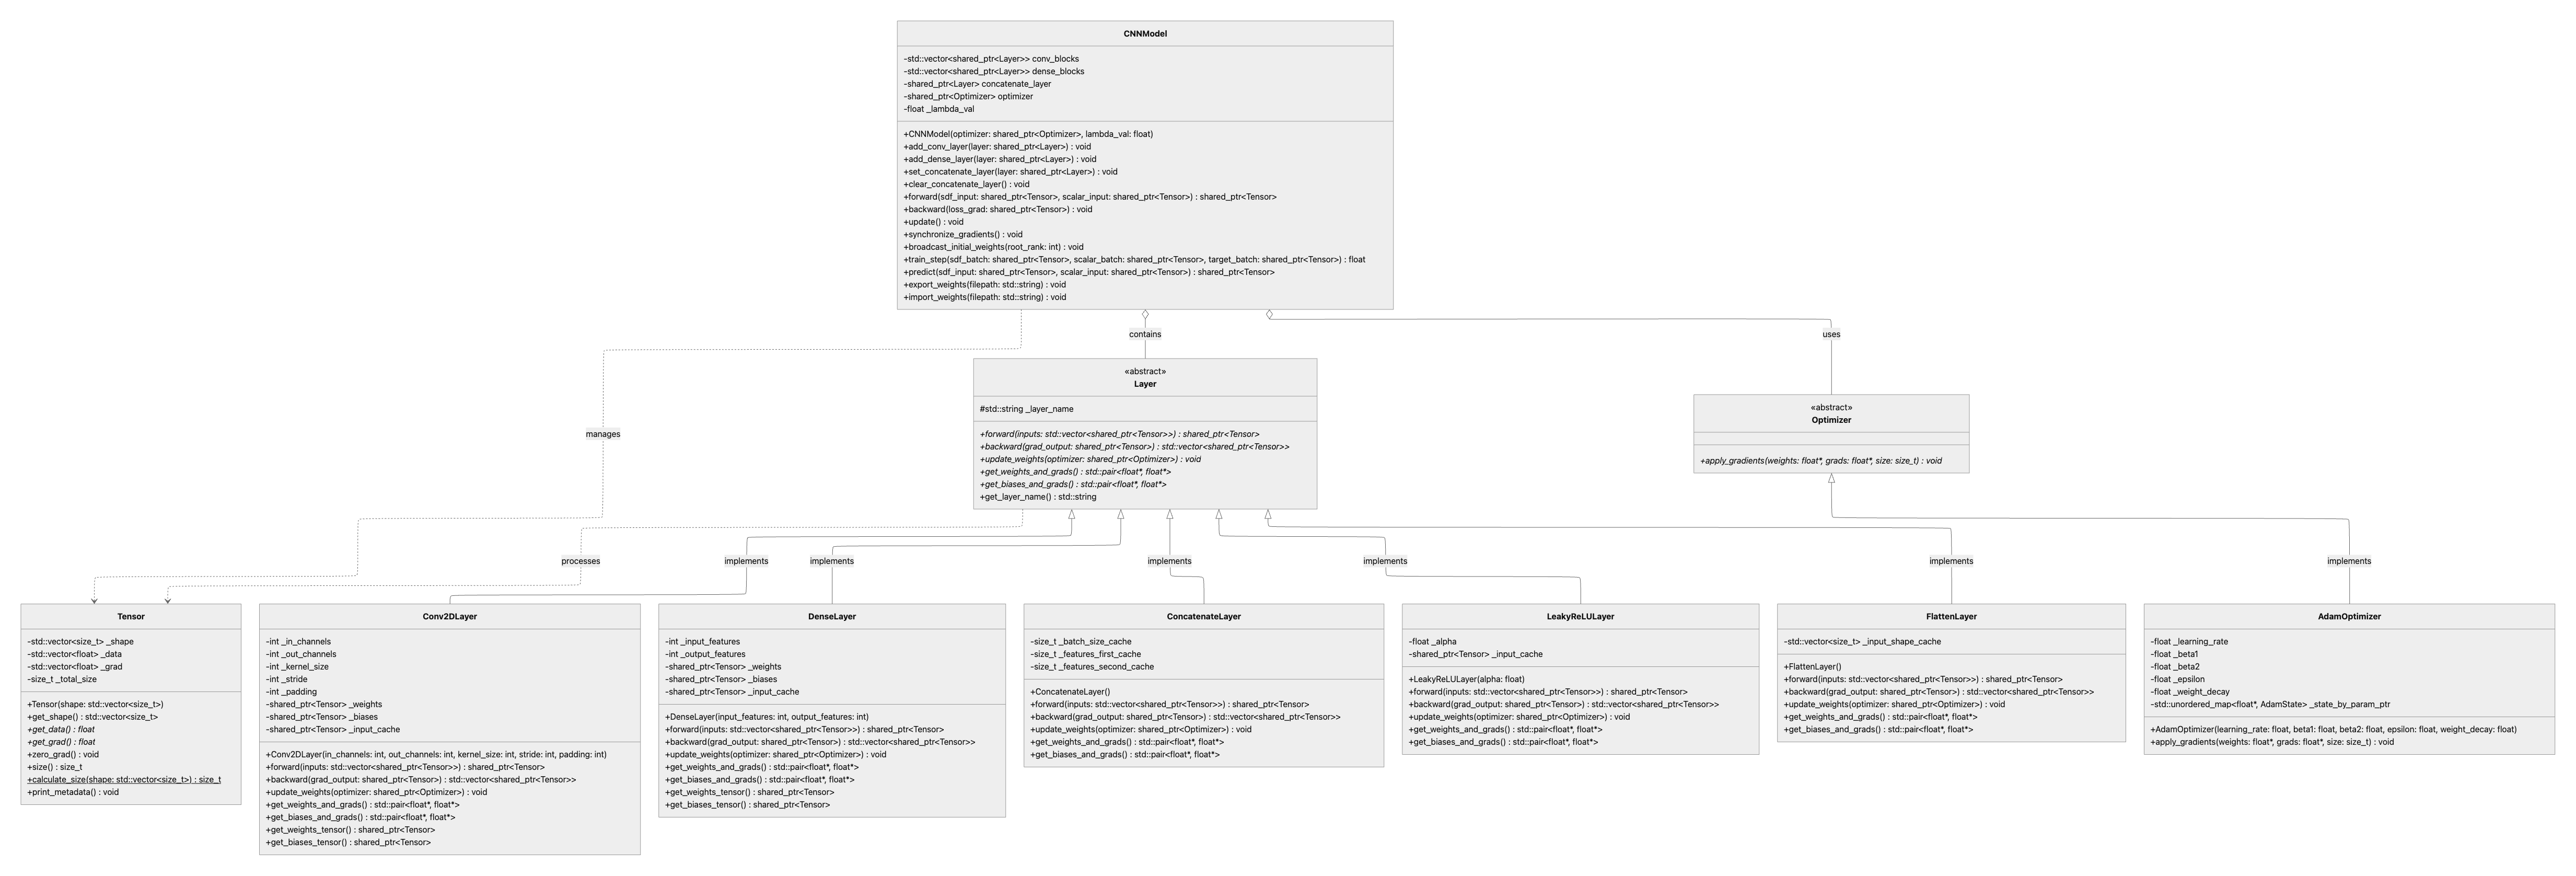
\includegraphics[width=1\linewidth]{Images/Chapter03/uml_diagram.png}
    \caption{UML class diagram illustrating the object-oriented design of the \cpp Convolutional Neural Network.}
    \label{fig:03_cnn_uml}
\end{figure}

In the following sections, we decide to highlight the most interesting implementations of these components, detailing key choices and memory optimization layouts, as well as providing an explanation of the core functions implemented.

\subsubsection{Geometric Preprocessing: SDF Generator}

The generation of the Signed Distance Function is encapsulated within the \texttt{SDFGenerator} class, which maps airfoil geometries to structured 2D tensors suitable for convolutional processing.\\

To maximize CPU cache efficiency and minimize cache misses during spatial calculations, boundary vertices are stored in a \texttt{std::vector<Point>}, where \texttt{Point} is a simple structure holding \texttt{x} and \texttt{z} coordinates. This choice creates a single contiguous array for the boundary data.\\

Upon initialization, the constructor ensures scale invariance (as detailed in Section \ref{sec:03_SDF}) by calling two private helper methods: \textbf{\texttt{computeCord()}} calculates the chord length $c$ using \texttt{std::hypot} to prevent numerical overflow\footnote{This function scales intermediate values before performing the sum of squares, avoiding the premature overflow or underflow that can occur when computing the norm directly as $\sqrt{\Delta x^2 + \Delta z^2}$} and \textbf{\texttt{normalizePoint()}} scales all vertex coordinates accordingly\footnote{This normalization step will be valuable for future implementations aimed at studying the effect of ice accumulation on the lift coefficient.}.\\

With a normalized boundary in place, the \texttt{SDFGenerator} computes the signed distance for each point on the target grid. This is achieved through a set of optimized geometric kernel functions:
\begin{itemize}
    \item[-] \textbf{\texttt{computeDistance(...) const}} calculates the minimum Euclidean distance from a grid point to a boundary segment (as it is shown in Equations \eqref{eq:03_orthogonal_projection} and \eqref{eq:03_clamping}). It includes a safety check for degenerate edges (where the two end-point of the segment coincide) to prevent division-by-zero errors;
    \item[-] \textbf{\texttt{getMinDistance(...) const}} iterates through all boundary edges of the airfoil, calling for each one \texttt{computeDistance} and returning the absolute minimum distance found. Additionally, we used \\\texttt{static\_cast<int>(airfoil.boundary.size())} to safely convert the unsigned vector size to a signed integer, preventing signed/unsigned comparison warnings;
    \item[-] finally, the \textbf{\texttt{windingAlgorithm(...) const}} implements the Winding Number Algorithm previously explained (Section \ref{sec:03_SDF}) to verify whether a grid point $p$ lies inside or outside the closed boundary. This is computed by analyzing edge crossings and using the 2D cross product (Equation \eqref{eq:cross_product})\footnote{Implemented through the \textbf{\texttt{crossProduct(Point p, Point a, Point b) const}} with each point passed by value, in order improve performance for small \texttt{structs} by allowing them to be passed directly in CPU registers, avoiding memory indirection.}, returning \texttt{true} if the point is inside the domain.
\end{itemize}
\vspace{2ex}

Once these values are computed for every grid point, the \textbf{\texttt{mappingToMatrix}} function converts the resulting 1D flattened SDF data into the required $150 \times 150$ 2D matrix format and writes it to a file, utilizing the \textbf{RAII (Resource Acquisition Is Initialization)} paradigm via \texttt{std::ofstream outfile(filename)} that automatically closes the file descriptor when \texttt{outfile} goes out of scope, in order to prevent system resource leaks in case of exceptions.\\

The most computationally intensive part of the process is executing these kernels for each one of the $150 \times 150 = 22,500$ points on the grid. This task is a classic example of an \textit{embarrassingly} parallel problem and it is implemented in the \texttt{generateTensorMPI} method, the details of which are provided in Section \ref{sec:03_parallelism}.

\subsubsection{Core abstractions and memory management}

To achieve high computational throughput while preserving a flexible design, the system introduces two core abstractions: a unified multi-dimensional tensor representation and a polymorphic layer interface.

\paragraph{Tensor}

The foundational data structure of our CNN implementation is the \texttt{Tensor} class, which manages both forward activation data (\texttt{\_data}) and backward gradients (\texttt{\_grad}) as multi-dimensional arrays of single-precision floating-point numbers.\\

First of all, the constructor \textbf{\texttt{Tensor(std::vector<size\_t> shape)}} initializes the shape descriptor and sets the \texttt{\_total\_size} member through a member \textbf{initializer list}. It pre-allocates and zero-initializes the storage vectors using \texttt{std::vector::resize}, that guarantees contiguous memory allocation. Direct access to this underlying memory is provided via the \texttt{get\_data()} and \texttt{get\_grad()} methods, which return raw pointers (\texttt{float*}) using the \texttt{.data()} member function.\\

Beyond raw pointer access, the class provides safe, native array-like indexing for flattened 1D elements through overloaded \texttt{operator[]} methods, offering both mutable and read-only (\texttt{const}-qualified) references. Utility functions are also optimized: gradient values are efficiently reset before each backward pass using the \texttt{std::fill} algorithm within the \texttt{zero\_grad()} method.\\

Furthermore, the total element count is computed by \texttt{calculate\_size()}, which is declared as a \texttt{static} method\footnote{This allows the method to be invoked without a class instance, for example, within a member initializer list.} and accepts a constant reference to avoid the overhead of copying the shape vector.\\

Finally, the class strictly adheres to \texttt{const} correctness, ensuring that utility methods like \texttt{print\_metadata()} are executed safely without modifying the object's internal state.

\paragraph{Layer}

The abstract base class \texttt{Layer}, defined in \texttt{Layer.hpp}, establishes a unified interface for all CNN components by leveraging runtime polymorphism to decouple the high-level network topology from the specific implementations of individual layers.\\

\textbf{Runtime polymorphism} is achieved through virtual functions and dynamic dispatch. When a class declares virtual methods, the compiler generates a virtual method table (\texttt{vtable}) containing pointers to these functions. Each object instance is implicitly equipped with a pointer (\texttt{vptr}) to its class's \texttt{vtable}. During execution, when a virtual method is called via a base class pointer, the program resolves the call dynamically: it dereferences the object's \texttt{vptr} to access the \texttt{vtable} and executes the overridden method corresponding to the actual derived type.\\

This mechanism is fundamental to our design. Rather than relying on conditional logic to handle the different mathematical operations, polymorphism allows the model to store and manage all layers uniformly within a single container (\texttt{std::vector<std::shared\_ptr<Layer>}). In addition, this design ensures high scalability and the effortless integration of new layer types simply by inheriting from the \texttt{Layer} base class.\\

Following the idea of implementing the polymorphism, we declared a virtual destructor \textbf{\texttt{\textasciitilde Layer() = default}}, ensuring that when a derived layer object is destroyed via a base class pointer, the derived class's destructor is executed, preventing resource leaks of dynamically allocated memory.\\

The core operations of the network are declared as pure virtual functions (indicated by the \texttt{= 0} suffix), which must be overridden by every concrete layer subclass. Specifically, we implemented:
\begin{itemize}
    \item[-] \textbf{\texttt{forward}}, that computes forward activations, and \textbf{\texttt{backward}}, that performs backpropagation, both accepting and returning \texttt{std::shared\_ptr} in order to guarantee automatic memory deallocation when the tensors are no longer needed;
    \item[-] \textbf{\texttt{get\_weights\_and\_grads()}} and \textbf{\texttt{get\_biases\_and\_grads()}} that returns \texttt{std::pair<float*, float*>} packaging the weight/bias arrays and their corresponding gradients into a single return value. Returning non-const pointers allows the optimizer to modify the parameter values directly in place.
\end{itemize}
\vspace{2ex}

Finally, architectural decoupling is achieved through a forward declaration of the \texttt{Optimizer} class; this resolves potential circular dependencies while allowing the \texttt{update\_weights(std::shared\_ptr<Optimizer>)} method to delegate parameter updates to external optimization algorithms seamlessly.

\subsubsection{Computational and activation layers}

The computational layers manage the network's mathematical transformations and contain all trainable parameters, while activation layers introduce the necessary non-linear activation boundaries.

\paragraph{DenseLayer}

The concrete \texttt{DenseLayer} class implements the fully-connected linear transformation $\mathbf{y} = W \mathbf{x} + \mathbf{b}$, where $W$ is the weight matrix and $\mathbf{b}$ is the bias vector, as described in details in the Section \ref{sec:03_dense_layer}.\\

First of all, the constructor \texttt{DenseLayer(int input\_features, int output\_features)} allocates the weight and bias tensors utilizing \texttt{std::make\_shared} rather than direct initialization via \\\texttt{std::shared\_ptr(new Tensor(...))}. While this last one forces two separate heap allocations\footnote{One for the object and one for its control block.}, \\\texttt{std::make\_shared} performs a \textbf{single contiguous memory allocation} for both the reference-counting control block and the managed \texttt{Tensor} object, in order to reduce heap fragmentation and improve CPU cache locality by keeping the control metadata and the tensor data adjacent in memory.\\

To ensure gradient stability at the start of training, the weights are initialized according to the \textbf{Xavier/Glorot scheme}, drawing from a uniform distribution bounded by $\pm\sqrt{6 / (N_{\text{in}} + N_{\text{out}})}$ using \texttt{std::default\_random\_engine} and \texttt{std::uniform\_real\_distribution<float>}.\\

During the \texttt{forward} pass, the input tensor is explicitly cached (\texttt{\_input\_cache}) to satisfy the mathematical requirements of backpropagation, as the input vector $\mathbf{x}$ must be retained to compute the weight updates as $\frac{\partial L}{\partial W} = \mathbf{x} \otimes \frac{\partial L}{\partial \mathbf{y}}$.\\

Moreover, the linear transformation $Y = X W^T + \mathbf{b}$ is evaluated through three nested loops:
\begin{itemize}
    \item[-] the outermost loop iterates over the batch size $b$;
    \item[-] the middle loop iterates over the output features $j$;
    \item[-] the innermost loop iterates over the input features $i$ to evaluate the dot product $Y_{b,j} = \sum_i X_{b,i} W_{j,i} + b_j$.
\end{itemize}
The weight matrix $W$ is stored in a transposed format of shape $(N_{\text{out}}, N_{\text{in}})$. This ensures that as the innermost loop increments its index over the input features, it accesses both the input tensor $X$ and the weight tensor $W$ with a unit stride. This design maximizes spatial locality, reduces cache misses, and enables the compiler to generate efficient SIMD vector instructions.\\

To conclude, also the \texttt{backward} method computes the gradients through three distinct sets of nested loops:
\begin{enumerate}
    \item the gradient with respect to the inputs is calculated as $dX_{b,i} = \sum_j dY_{b,j} W_{j,i}$. In this loop structure, the weight matrix is traversed column-wise, resulting in non-contiguous memory access;
    \item the gradient with respect to the weights is accumulated as $dW_{j,i} = \sum_b dY_{b,j} X_{b,i}$ using loops over $j$, $i$, and the batch dimension $b$. The innermost loop iterates over $b$, calculating the outer product of the output gradients and cached inputs;
    \item the gradient with respect to the biases is accumulated as $dB_j = \sum_b dY_{b,j}$ by summing the output gradients across all batch elements for each output feature.
\end{enumerate}

\paragraph{LeakyReLULayer}

The concrete \texttt{LeakyReLULayer} class implements homonymous element-wise activation function shown in Equation \eqref{eq:03_leaky_relu}. The negative slope parameter $\alpha$ is configured into the constructor \texttt{LeakyReLULayer(float alpha = 0.05f)}.\\

The interesting thing in this code is the use of the ternary operator:
\begin{itemize}
    \item[-] in the \texttt{forward} method, the element-wise activation is evaluated inside a contiguous loop using raw pointers \texttt{out\_ptr[i] = (in\_ptr[i] > 0.0f) ? in\_ptr[i] : \_alpha * in\_ptr[i]};
    \item[-] in the \texttt{backward} method, that is used to evaluate the gradient with respect to the input by scaling the output gradient as shown in Equation \eqref{eq:03_derivative_leaky_relu}, implemented as \texttt{din\_ptr[i] = dout\_ptr[i] * ((cache\_ptr[i] > 0.0f) ? 1.0f : \_alpha)}.
\end{itemize}
Because the derivative of the activation function is conditioned on the sign of the original input activations, caching the forward input tensor inside \texttt{\_input\_cache} is necessary to retrieve the values during the backward pass.\\

To conclude this class, because the activation layer contains no learnable parameters, the overridden method \texttt{update\_weights} is implemented as a no-op. Moreover, the parameter accessors \texttt{get\_weights\_and\_grads()} and \texttt{get\_biases\_and\_grads()} return a pair of type-safe null pointers, \texttt{\{nullptr, nullptr\}}.

\paragraph{Conv2DLayer}
\label{sec:03_conv}

The concrete \texttt{Conv2DLayer} class extends the abstract \texttt{Layer} interface to perform 2D spatial convolutions on four-dimensional tensors, which logically represent \textbf{batch samples, channels, height and width}.\\

Upon instantiation, the constructor initializes the convolutional kernels using a \textbf{Gaussian Xavier scheme} to ensure variance stability across deep network layers. The standard deviation for this distribution is computed as $\sigma = \sqrt{2 / (F_{\text{in}} + F_{\text{out}})}$, where the fan-in and fan-out dimensions are defined as $F_{\text{in}} = C_{\text{in}} \times K^2$ and $F_{\text{out}} = C_{\text{out}} \times K^2$, with $K$ denoting the kernel size.\\

During the \texttt{forward} pass, the spatial dimensions of the output tensor are explicitly calculated using Equation \eqref{eq:03_convol} and the resulting tensor is allocated contiguously via \texttt{std::make\_shared}. Because the system flattens all multi-dimensional tensors into 1D contiguous vectors for optimal memory layout, the layer utilizes a private inline helper function, \texttt{idx4}, to resolve 4D indices to 1D offsets. This enforces a strict row-major mapping:
\begin{equation}
    \text{Offset}(a, b, c, d) = \left[ \left( a \times \text{dim}_b + b \right) \times \text{dim}_c + c \right] \times \text{dim}_d + d
\end{equation}
where $a, b, c, d$ represent the target indices across the batch, channel, and spatial dimensions.\\

The forward convolution operation is executed through seven-nested loop. The outer four loops iterate over the batch elements $n$, output channels $oc$ and spatial output coordinates $oh$ and $ow$, while the inner three loops traverse the input channels $ic$ and kernel dimensions $kh$ and $kw$. To handle boundaries without incurring the overhead of allocating memory for physical zero-padding, the implementation uses implicit padding. Source coordinates are dynamically evaluated at each step as $ih = oh \times S + kh - P$ and $iw = ow \times S + kw - P$:
\begin{itemize}
    \item[-] if these fall outside the input boundaries, the multiplication is safely bypassed using a \texttt{continue} statement;
    \item[-] otherwise, the flattened indices are retrieved via \texttt{idx4}, and the kernel-input products are accumulated into a running sum initialized with the appropriate channel bias.
\end{itemize}
\vspace{2ex}

Finally, the \texttt{backward} method evaluates gradients using two distinct loop structures:
\begin{enumerate}
    \item[-] the first structure computes the parameter gradients: the bias gradient ($dB$) aggregates the output gradients directly, while the weight gradient ($dW$) accumulates the product of the output gradients and the cached forward inputs;
    \item[-] the second structure computes the gradient with respect to the input ($dX$) by performing a full convolution between the output gradients and the flipped kernel filters. To achieve this, the loop accesses the weights using inverted spatial coordinates:
    \begin{equation}
        kh_{\text{orig}} = K - 1 - kh, \quad kw_{\text{orig}} = K - 1 - kw
    \end{equation}
\end{enumerate}

\subsubsection{Structural Layers}

The \textbf{structural layers} are parameter-free components designed to rearrange and route data tensors across the branches of the network.

\paragraph{FlattenLayer}

The \texttt{FlattenLayer} class extends the base \texttt{Layer} interface to perform a logical reshaping of the 4D feature maps (generated by the convolutional branch) into a 2D tensor suitable for the subsequent \texttt{ConcatenateLayer}.\\

The \texttt{forward} method calculates the flattened size $F = C \times H \times W$ and allocates a 2D output tensor of shape $[B \times F]$ via \texttt{std::make\_shared}. Since the flatten operation is basically a reshape, the data is copied from the input to the output tensor sequentially in a single loop, preserving the element order across contiguous memory arrays.\\

The \texttt{backward} method receives the 2D gradient tensor \texttt{grad\_output} (of shape $[B \times F]$), validates the batch size consistency, allocates a 4D gradient tensor matching the cached shape \texttt{\_input\_shape\_cache}\footnote{This member attribute of type \texttt{std::vector<size\_t>} preserves the original spatial dimensions ($C \times H \times W$) to reconstruct and propagate the gradient back.} and performs the inverse sequential copy \texttt{grad\_in\_ptr[i] = grad\_out\_ptr[i]}, reconstructing the 4D gradient layout for the preceding convolutional layer.

\paragraph{ConcatenateLayer}

The \texttt{ConcatenateLayer} class is used to obtain a single tensor that combines the information from the \textbf{Convolutional Layer} and the scalar values of the Reynolds number and angle of attack.\\

Beyond the mathematical formalism about the shape of the matrices described in a detailed way in Section \ref{sec:03_struct_layer}, the merge operations are implemented with nested loops:
\begin{itemize}
    \item[-] the outer loop iterates over the batch size $n$, computing the row offsets for the first input \\(\texttt{n * \_features\_first\_cache}), the second input (\texttt{n * \_features\_second\_cache}) and the output (\texttt{n * (\_features\_first\_cache + \_features\_second\_cache)});
    \item[-] two inner loops then copy the data, ensuring row-wise contiguous layout. 
\end{itemize}
\vspace{2ex}
During the \texttt{backward} method, this operation is inverted. The layer receives a combined gradient tensor of shape $[B \times (D_1 + D_2)]$ and must route the gradients back to their respective origins, reversing the copy logic: for each batch element, it copies the first $D_1$ components of the output gradient to the first input gradient buffer and the remaining $D_2$ components to the second input gradient buffer. Both elements are then returned in a standard vector \texttt{\{grad\_first, grad\_second\}}.

\subsubsection{Training pipeline, loss and optimizers}

The network's optimization and training pipeline is coordinated by mathematical loss functions and state-tracking optimization solvers.

\paragraph{Loss}

Unlike the object-oriented structure of the computational layers, the \textbf{physics-informed loss function} and its corresponding gradient are implemented as non-member utilities within the \texttt{Loss} namespace. This design choice avoids the overhead of object instantiation and maintains a functional style for stateless operations.\\

In the \texttt{forward} method\footnote{That accepts predictions, targets and angles of attack (\texttt{alphas}) tensors as \texttt{const std::shared\_ptr<Tensor>\&}.}, the composite physics-informed loss, described in Section \ref{sec:03_loss}, is computed in a single loop using raw pointers retrieved via \texttt{get\_data()} to ensure contiguous memory traversal. When computing the physics-informed penalty, the masking logic from Equation \eqref{eq:03_mask} is applied: the linear regime limit is saved in an anonymous namespace at the beginning of the file, in order to restrict the scope of this constant. The average data and physics terms are computed and normalized by the number of elements using \texttt{static\_cast<float>(n)}\\

Finally, the \texttt{backward} method is implemented in a similar way.

\paragraph{Optimizer and Adam Optimizer}

Similar to the layer architecture, the optimization logic is strictly decoupled from the neural network topology via an abstract \texttt{Optimizer} base class. This unified interface ensures that different numerical solvers can be swapped seamlessly, exposing a single pure virtual function (\texttt{apply\_gradients(float* weights, float* grads, size\_t size)}) to handle dynamic dispatch interface that must be implemented by concrete subclasses.\\

The only concrete implementation of this interface is the \texttt{AdamOptimizer}, which executes the \textbf{Adaptive Moment Estimation} algorithm detailed in Section \ref{sec:03_adam}.\\

To map specific weight and bias arrays to their corresponding optimization states without coupling the layers to the optimizer, the class utilizes a parameter-to-state lookup map as \texttt{std::unordered\_map<float*, AdamState> \_state\_by\_param\_ptr}\footnote{Where \texttt{AdamState} is a private structure that contains the first moment vector \texttt{std::vector<float> m}, the second moment vector \texttt{std::vector<float> v}, and an unsigned integer \texttt{timestep} to keep track of the parameter update steps.}, that provides average constant-time $\mathcal{O}(1)$ lookup complexity. Since weight and bias arrays are allocated once and reside in contiguous memory locations throughout the lifetime of the network, their raw memory addresses (\texttt{float*}) serve as unique keys. This pointer-based hashing avoids the overhead of index-based tracking or string-based lookups and enables on-the-fly initialization of the \texttt{AdamState} upon the first optimization step.

\paragraph{CNNModel}
\label{sec:03_CI_CNN}

The concrete class \texttt{CNNModel} coordinates the execution, training and state management of the entire neural network. It aggregates the layers of the convolutional branch and the dense branch, manages feature fusion, interfaces with the optimizer and implements utilities for distributed data-parallel training and weight serialization.\\

The \texttt{forward} method propagates input tensors sequentially through the model. To maximize efficiency, the iteration over the layer containers (\texttt{conv\_blocks} and \texttt{dense\_blocks}) utilizes \texttt{const auto\&}, thereby avoiding the performance overhead associated with incrementing reference counters on the underlying shared pointers. Conversely, the \texttt{backward} method employs reverse iterators to correctly propagate gradients upstream in strict accordance with the chain rule.\\

Another interesting detail is that in the \texttt{update} method gradient values are clipped to the interval $[-1.0, 1.0]$ to prevent gradient explosion\footnote{This choice has been made after training the model for the first time, where we have noticed very strong fluctuations of the loss value during the training process.}. This is executed via a local lambda function (\texttt{clip\_layer}) containing a nested \texttt{clip\_tensor} lambda, which directly modifies the elements in-place using standard pointer-based loops. \\

Whenever layer-specific parameters must be accessed for weight updates, gradient synchronization, or serialization, the model dynamically resolves the abstract base pointer types through runtime downcasting via \texttt{std::dynamic\_pointer\_cast} (e.g., casting from \texttt{std::shared\_ptr<Layer>} to \texttt{std::shared\_ptr<Conv2DLayer>}).\\

Finally, the model implements binary weight export and import methods using \texttt{std::ofstream} and \texttt{std::ifstream}, opened with the \texttt{std::ios::binary} flag. Binary data is written and read directly via type-unsafe low-level operations utilizing \texttt{reinterpret\_cast<const char*>} and \texttt{reinterpret\_cast<char*>} to map raw byte buffers, which minimizes I/O latency. During the import phase, after reading the shapes and element counts from the file, weight vectors are populated using \texttt{std::move} (from the \texttt{<utility>} header) to transfer the ownership of heap-allocated arrays into the target structures, bypassing expensive memory allocation and copying. To illustrate this efficient binary format, Table \ref{tab:weights_header_example} details the layout of the file header and the metadata corresponding to the initial \texttt{Conv2DLayer}.

\begin{table}[h!]
  \centering
  \caption{Example layout of the binary weight file header, showing the global count of layers followed by the name and weight/bias tensor metadata of the first layer (\texttt{Conv2DLayer}).}
  \label{tab:weights_header_example}
  \begin{tabular}{lll}
    \hline
    Byte Offset & Field Name & Value / Example \\
    \hline
    \texttt{0x00--0x07}   & Total layers in model ($N_{\text{layers}}$) & \texttt{8} \\
    \texttt{0x08--0x0F}   & Layer name length ($L_{\text{name}}$) & \texttt{39} \\
    \texttt{0x10--0x36}   & Layer name string & \texttt{"Conv2DLayer(1,8,5, stride=5, padding=0)"} \\
    \texttt{0x37}         & Weights presence flag & \texttt{true} (\texttt{0x01}) \\
    \texttt{0x38--0x3F}   & Weights tensor rank ($R_W$) & \texttt{4} \\
    \texttt{0x40--0x5F}   & Weights tensor shape & \texttt{[8, 1, 5, 5]} \\
    \texttt{0x60--0x67}   & Total weights count ($N_W$) & \texttt{200} \\
    \texttt{0x68--0x387}  & Weights raw data & \texttt{[-0.0125, 0.0841, \dots]} \\
    \texttt{0x388}        & Biases presence flag & \texttt{true} (\texttt{0x01}) \\
    \texttt{0x389--0x390} & Biases tensor rank ($R_B$) & \texttt{1} \\
    \texttt{0x391--0x398} & Biases tensor shape & \texttt{[8]} \\
    \texttt{0x399--0x3A0} & Total biases count ($N_B$) & \texttt{8} \\
    \texttt{0x3A1--0x3C0} & Biases raw data & \texttt{[0.0, 0.0, \dots]} \\
    \hline
  \end{tabular}
\end{table}

\subsubsection{Data Pipelines: \texttt{NPZDataLoader}}

The \texttt{NPZDataLoader} class manages the retrieval, normalization, and partitioning of datasets stored in the compressed NumPy (\texttt{.npz}) format. This format was explicitly selected because it packages multiple named multidimensional arrays within a single ZIP archive, acting as an efficient bridge between Python-based preprocessing scripts (such as \texttt{build\_dataset.py}) and the \cpp training pipeline without the severe parsing overhead of text-based formats like CSV.\\

Specifically, the dataset is structured into four core arrays:
\begin{itemize}
    \item[-] \texttt{X\_sdf}, representing the $150 \times 150$ SDF of the airfoil geometries;
    \item[-] \texttt{X\_scalars}, storing the Reynolds number ($\mathrm{Re}$) and the angle of attack ($\alpha$);
    \item[-] \texttt{Y\_cl}, containing the ground-truth lift coefficient ($C_L$) labels computed from the Navier-Stokes simulations;
    \item[-] \texttt{metadata}, containing the specific NACA airfoil profile labels.
\end{itemize}
This class provides a complete input pipeline, converting these raw data arrays into normalized, formatted tensor batches for network training.\\

To import the data without introducing heavy external \cpp NumPy parsing libraries, the internal reading method establishes a read-only POSIX pipe to execute a brief Python script, that utilizes Python's native numpy library to load the specified array, converts it to raw single-precision bytes and streams the output directly to the standard output. The \cpp program then intercepts this byte stream, reading it sequentially into a standard vector buffer before safely closing the process and verifying its exit status.\\

Once the arrays are loaded into memory, the constructor applies Z-score standardization across the SDF, scalar parameters and target lift coefficients, to prevent numerical instability during the training phase. Then, the class handles the sequential feeding of this data during training. The batching process partitions the normalized dataset into mini-batches by maintaining an internal cursor that tracks the current read position. For each requested batch, it allocates new tensor objects and utilizes standard library copying algorithms to transfer the exact slice of data from the internal buffers to the newly created tensors.

\subsubsection{Main execution of the CNN}

The main execution entry point of the neural network workflow is defined in \texttt{main.cpp}. It coordinates the loading of datasets, the structural composition of the CNN layers and the training and validation loops over successive epochs.\\

The program begins by instantiating the training and testing pipelines using \texttt{NPZDataLoader} to load the compressed NumPy datasets. It then creates a shared instance of the \texttt{AdamOptimizer} wrapped in a \texttt{std::shared\_ptr} via \texttt{std::make\_shared} with a designated learning rate of $10^{-5}$. This optimizer is passed to initialize the \texttt{CNNModel} instance.\\

The architecture of the neural network is composed using the model's builder methods:
\begin{enumerate}[itemsep=2ex, topsep=2ex]
    \item the convolutional branch is constructed by adding a \texttt{Conv2DLayer} with 1 input channel, 8 output channels, a $5 \times 5$ kernel, and a stride of 5, followed by a \texttt{LeakyReLULayer} (with an activation slope $\alpha = 0.05$) and a \texttt{FlattenLayer} to reduce the spatial feature maps to a one-dimensional representation of size 7200;
    \item the feature fusion stage is enabled by registering a \texttt{ConcatenateLayer} via \texttt{set\_concatenate\_layer()}, which merges the geometry features with the two physical flow parameters (Reynolds number and angle of attack);
    \item the fully-connected regression head is built using three sequential \texttt{DenseLayer}s of dimensions $7202 \to 128$, $128 \to 64$, and $64 \to 1$, separated by \texttt{LeakyReLULayer} activations, resulting in a single scalar prediction representing the lift coefficient ($C_L$).
\end{enumerate}
\vspace{2ex}
The training process iterates for 100 epochs. Within each epoch, it resets the data loaders and processes the dataset in mini-batches. For each batch, it invokes \texttt{train\_step} on the model instance to run the forward pass, evaluate the PINN loss function, compute parameter gradients via backpropagation and update the weights. After the training phase of each epoch, it runs a validation pass by propagating the validation samples through the network via \texttt{forward()} to monitor generalization and check for overfitting by computing the MSE against the validation targets.

% ===================================================================
% PARALLELISM AND SCALABILITY
% ===================================================================

\subsection{Parallelism}
\label{sec:03_parallelism}

To achieve high-performance capabilities and scale the computational workflow to large-scale grids and datasets, the codebase employs distributed-memory parallelism using the \textbf{Message Passing Interface (MPI)} standard. The parallelization strategy is implemented at two distinct stages: the geometric preprocessing phase (for parallel SDF generation) and the neural network training phase (for distributed data-parallel training).

\subsubsection{Parallel SDF Generation}

The computation of the SDF, as described in Section \ref{sec:03_SDF}, is an embarrassingly parallel task, since the evaluation of the signed distance for each point on the $150 \times 150$ grid is independent of all other points.\\

To do this, upon initializing the MPI environment via \texttt{MPI\_Init}, the total number of grid points ($N_{\text{total}} = 22,500$) is partioned by the communicator size ($S$, retrieved using \texttt{MPI\_Comm\_size}). Because there could be some cases where $N_{\text{total}}$ is not perfectly divisible by $S$, the remainder ($R = N_{\text{total}} \bmod S$) is distributed among the first $R$ processes\footnote{This partitioning guarantees perfect load balancing, as the workload of any two processes differs by at most a single grid point.}. Each process (with rank ID $r$, retrieved via \texttt{MPI\_Comm\_rank}) computes its local count and offset as:
\begin{equation}
    N_{\text{local}} = \lfloor N_{\text{total}} / S \rfloor + \mathbb{I}(r < R)\quad\text{and}\quad O_{\text{local}} = r \lfloor N_{\text{total}} / S \rfloor + \min(r, R)
\end{equation}
where $\mathbb{I}$ is the indicator function.\\

Each process independently computes the SDF values for its assigned local grid points. To reconstruct the complete 2D matrix, the local chunks must be gathered into a global vector of size $N_{\text{total}}$, using \texttt{MPI\_Allgatherv}, which performs a vector gather-to-all communication. The collective call requires \texttt{recvcounts}, which stores the number of elements expected from each rank, and \texttt{displs}, which specifies the starting byte displacement of each segment in the global buffer. \texttt{MPI\_Allgatherv} ensures that all processes receive the full SDF image.\\

Finally, the root process (rank 0) writes the complete matrix to disk via the \texttt{mappingToMatrix} method, while other ranks proceed to the next file or terminate safely via \texttt{MPI\_Finalize}.

\subsubsection{Distributed Data-Parallel Training}

The training of the Convolutional Neural Network is parallelized in \texttt{CNN/main.cpp} and \texttt{CNNModel.cpp} using a data-parallel training strategy to scale to large datasets and decrease training epoch time.\\

In \texttt{CNN/main.cpp}, data parallelism is implemented by distributing the training batch across multiple processes. The global mini-batch size is scaled according to $B_{\text{global}} = B_{\text{local}} \times S$, with a local batch size of $B_{\text{local}} = 64$. To prevent redundant memory duplication, each process uses a custom \texttt{slice\_batch\_tensor} method to extract only its specific segment of the global dataset, beginning at the index offset $r \times B_{\text{local}}$.\\

To guarantee consistent optimization across the distributed environment, the training pipeline enforces MPI synchronization at three critical stages:
\begin{enumerate}[itemsep=2ex, topsep=2ex]
    \item initially, the root process generates the network weights and distributes them to all other ranks using \texttt{MPI\_Bcast} on the raw tensor buffers, ensuring an identical starting state\footnote{With all the weights initialized to the same value.} across the entire communicator;
    \item during the backpropagation phase, each process computes gradients based on its local batch slice. Before applying the Adam optimization step, these local gradients are aggregated via an in-place \texttt{MPI\_Allreduce} operation. By utilizing the \texttt{MPI\_SUM} operator directly on the existing memory buffers, the system efficiently avoids redundant data allocations. The accumulated gradients are then divided by the total number of processes $S$ to compute a global average, which guarantees that every rank applies the exact same mathematical update to its local parameters;
    \item finally, at the conclusion of each epoch, the local training losses, validation losses, and processed sample counts are gathered back to the root process via \texttt{MPI\_Reduce}, allowing it to calculate and report the consolidated global statistics.
\end{enumerate}

% ===================================================================
% RESULTS
% ===================================================================

\subsection{Results}

Given the significant model size of 930,513 trainable parameters, performing the training process on standard personal computers was computationally impractical within a reasonable timeframe. To overcome this limitation, the training was conducted on the high-performance computing (HPC) resources of the \textbf{CINECA Leonardo cluster}. Specifically, we utilized a full single node configured with two Intel Xeon Platinum 8480+ (Sapphire Rapids) processors, providing a total of 112 physical cores, backed by 512 GiB of DDR5 RAM operating at 4800 MHz. This hardware acceleration reduced the total execution time from several hours to approximately five minutes.\\

\begin{lstlisting}[style=bashstyle,
  caption={SLURM run script for CNN training (\texttt{run\_cnn.sh}).},
  label={lst:job_run}]
#!/bin/bash
#SBATCH --job-name=cnn_training
#SBATCH --account=EUHPC_D35_025
#SBATCH --partition=dcgp_usr_prod
#SBATCH --nodes=1
#SBATCH --ntasks-per-node=1
#SBATCH --cpus-per-task=112
#SBATCH --time=01:00:00
#SBATCH --output=cnn_%j.out
#SBATCH --error=cnn_%j.err


cd /leonardo/home/userexternal/gdonnine/CNN/Ice_acceleration_model_on_airplane_wing/CNN

module purge
module load python/3.11.7
module load gcc/11.3.0
module load intel-oneapi-compilers
module load intel-oneapi-mpi

srun ./cnn_mpi_executable
\end{lstlisting}

The network was trained for 100 epochs on a synthetically generated dataset of 2D SDF, representing five \textbf{symmetric NACA airfoil profiles} (NACA 0006, 0008, 0010, 0012 and 0018) across varying angles of attack ($\alpha$) and Reynolds numbers ($\mathrm{Re}$). Partitioned via an 80/20 split, the dataset yielded 1,713 training samples and 429 validation samples\footnote{All of which have been made publicly available on \href{https://www.kaggle.com/datasets/giulioenzodonninelli/sdf-symmetric-airfoil-high-reynolds-number}{\textcolor{blue}{Kaggle}}}.

\paragraph{Initial Unstable Training Run}

In our first training attempt, we adopted a standard learning rate of $10^{-3}$, without applying input feature normalization or gradient clipping. This configuration resulted in severe numerical instability during the optimization process. As illustrated in Figure \ref{fig:incorrect_training}, the training and validation losses exhibit chaotic, erratic oscillations, fluctuating wildly by over seven orders of magnitude (ranging from $10^{-1}$ to $10^6$ in log scale). The presence of massive loss spikes\footnote{Such as the prominent peaks around epochs 40, 60, 70 and 85.} is a clear indicator of exploding gradients. Without gradient clipping, large backpropagated gradients led to excessive parameter updates, pushing the weights into unstable regions of the loss landscape and preventing the optimizer from settling into a local minimum.

\begin{figure}[h!]
  \centering
  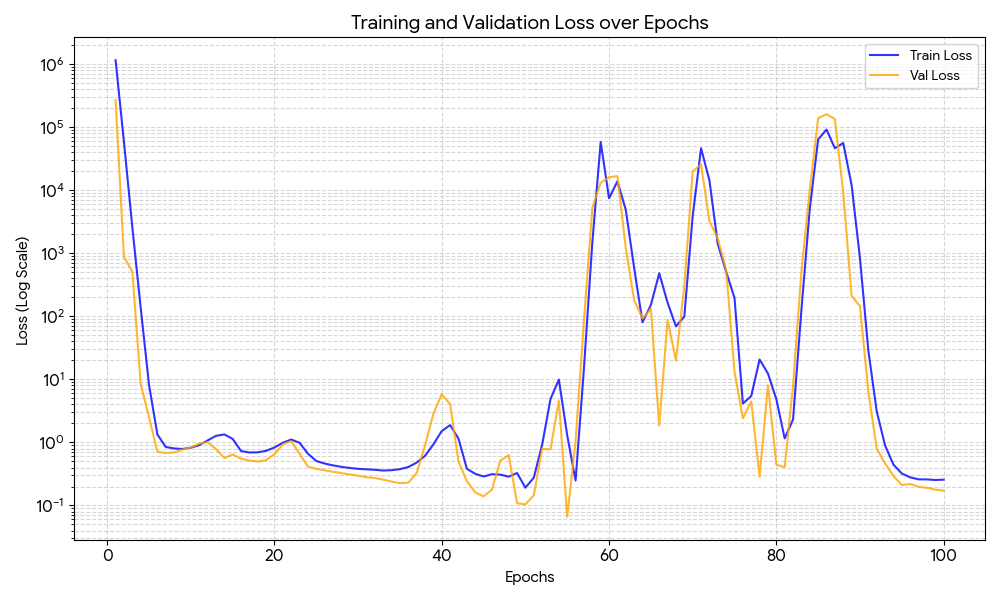
\includegraphics[width=0.70\linewidth]{Images/Chapter03/Incorrect_training.png}
  \caption{Log-scale evolution of the training and validation losses over 100 epochs during the initial unstable training attempt. The extreme oscillations and sudden spikes up to $10^6$ highlight the numerical instability caused by an excessively high learning rate and the absence of gradient clipping or feature normalization.}
  \label{fig:incorrect_training}
\end{figure}

\paragraph{Optimized Successful Training Run}

To resolve the numerical instability and ensure smooth convergence, three key modifications were implemented in the training pipeline:
\begin{enumerate}
    \item the Adam optimizer's learning rate ($\eta$) was reduced from $10^{-3}$ to $10^{-5}$;
    \item standard Z-score normalization was applied during the data-loading phase to scale the inputs (SDF and physical scalars) and targets (lift coefficients) to zero-mean and unit-variance;
    \item gradient clipping was enabled in the update phase to clamp all gradient components strictly within the interval $[-1.0, 1.0]$ (as detailed in Section \ref{sec:03_CI_CNN}).
\end{enumerate}
These modifications successfully stabilized the training trajectory.\\

As shown in Figure \ref{fig:correct_training}, the loss curves exhibit highly stable, monotonic convergence. The left plot (Full View) shows the rapid decay of the loss during the initial epochs, indicating that the network quickly learned the dominant physical relationships. The right plot (Zoomed View, Epochs 5-100) highlights the smooth, continuous reduction of both training and validation losses, with no signs of overfitting. The validation loss consistently tracks slightly lower than the training loss; this is a common characteristic when model regularization (such as L2 weight decay) is active during training or when the z-score normalization effectively centers the distribution of test cases.\\

This optimized training process completed in likely 5 minutes and 11 seconds, achieving a final training loss of 0.0104216 and a validation loss of 0.00784775, demonstrating both the efficiency and accuracy of our implementation.

\begin{figure}[h!]
  \centering
  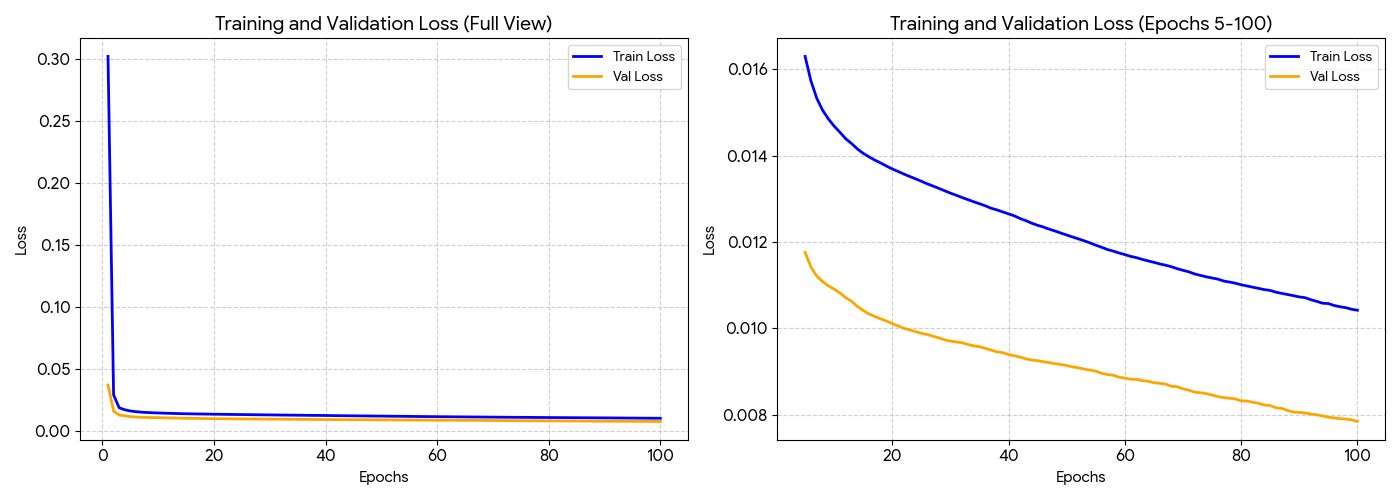
\includegraphics[width=0.85\linewidth]{Images/Chapter03/Correct_training.png}
  \caption{Evolution of training and validation losses for the optimized training run. The full view (left) illustrates the rapid initial convergence, while the zoomed-in view from epoch 5 to 100 (right) highlights the smooth, monotonic decrease of both metrics, confirming the effectiveness of Z-score normalization and gradient clipping.}
  \label{fig:correct_training}
\end{figure}